\section{Análisis de resultados}
Se tiene la Siguiente tabla de datos tomados para cierta concentración

% Create a Table of data centered
\begin{table}[h]
    \label{tab:data}
    \centering
    \begin{tabular}{|c|c|c|}
        \hline
        n & Concentración $C$ (M) & Absorbancia $A$\\
        \hline
        1 & $0.00008$ & $0.124$ \\
        \hline
        2 & $0.00016$ & $0.239$ \\
        \hline
        3 & $0.00040$ & $0.614$ \\
        \hline
        4 & $0.00080$ & $1.160$ \\
        \hline
    \end{tabular}
    \caption{Datos tomados para $\mathrm{K Mn O_4}$ en aguas residuales del río Piura}
\end{table}

se tiene el Siguiente gráfico
\begin{figure}[H]
    \centering
    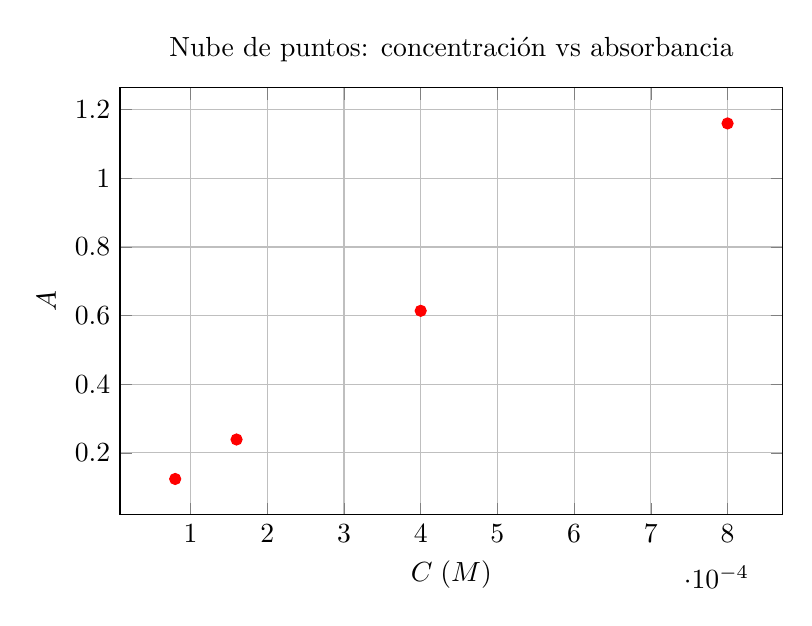
\begin{tikzpicture}
        \begin{axis}[
            grid=both,
            xlabel={$C\;(\text{M})$},
            ylabel={$A$},
            title={Nube de puntos: concentración vs absorbancia},
            width=10cm,
            height=7cm,
            ticklabel style={/pgf/number format/fixed},
        ]
        \addplot[
            only marks,
            mark=*,
            color=red,
            mark size=2pt
        ] coordinates {
            (0.00008, 0.124)
            (0.00016, 0.239)
            (0.00040, 0.614)
            (0.00080, 1.160)
        };
        \end{axis}
    \end{tikzpicture}
\end{figure}

Ahora utilizamos el método de mínimos cuadrados para calcular
la recta, donde

\begin{gather*}
    S_x = \sum_{i=0}^{n} x_i, \quad
    S_y = \sum_{i=0}^{n} y_i, \quad
    S_{xy} = \sum_{i=0}^{n} x_i y_i, \quad
    S_{xx} = \sum_{i=0}^{n} x_i^2 \\
    b = \frac{n S_{xy} - S_x S_y}{n S_{xx} - S_x^2}, \quad
    a = \frac{S_y - b S_x}{n}\\
    \mathscr{L}: y = a + bx
\end{gather*}

Donde $y$ es la absorbenta y $x$ la concentración.

De los datos de la tabla~\ref{tab:data} tenemos:
\begin{align*}
    S_x &= 0.00008 + 0.00016 + 0.00040 + 0.00080 = 0.00144\\
    S_y &= 0.124 + 0.239 + 0.614 + 1.160 = 2.137\\
    S_{xy} &= 0.00008 \times 0.124 + 0.00016 \times 0.239 \\
    &+ 0.00040 \times 0.614 + 0.00080 \times 1.160 = 0.00122176 \\
    s_x^2 &= 0.00008^2 + 0.00016^2 + 0.00040^2 + 0.00080^2 = 8.32\times10^{-7}\\ 
\end{align*}

Entonces el valor de $b$ será:
\begin{equation*}
    b = \frac{4 \times 0.00122176 - 0.00144 \times 2.137}{4\cdot8.32\times10^{-7} - 0.00144^2} = 1442.72959
\end{equation*}

Y el de $a$:
\begin{equation*}
    a = \frac{2.137 - 1442.72959 \times 0.00144}{4} = 0.01486 
\end{equation*}

Así la ecuación de la recta es: 
\begin{gather*}
    \mathscr{L}: y = 0.01487 + 1442.72959 x
\end{gather*}

% Coef Relation
El coeficiente de correlación lineal \(r\) en notación de sumas es
\[
r=\frac{n S_{xy}-S_x S_y}{\sqrt{\big(n S_{xx}-S_x^2\big)\big(n S_{yy}-S_y^2\big)}}.
\]

Sustituyendo:
\[
\begin{aligned}
r &=\frac{4(0.00122176)- (0.00144)(2.137)}
{\sqrt{\big(4(8.32\times10^{-7})-(0.00144)^2\big)\big(4(1.795092999)- (2.137)^2\big)}}\\[6pt]
&\approx 0.9995008146.
\end{aligned}
\]

Finalmente,
\[
\boxed{R^2 = r^2 \approx (0.9995008)^2 \approx 0.9990019 \approx 0.9990.}
\]

\noindent Esto significa que aproximadamente el \(99.90\%\) de la variabilidad de \(A\) queda explicada por la concentración \(C\) mediante la recta de ajuste.
% end Coef relation

\bigskip
\begin{figure}[H]
\centering
 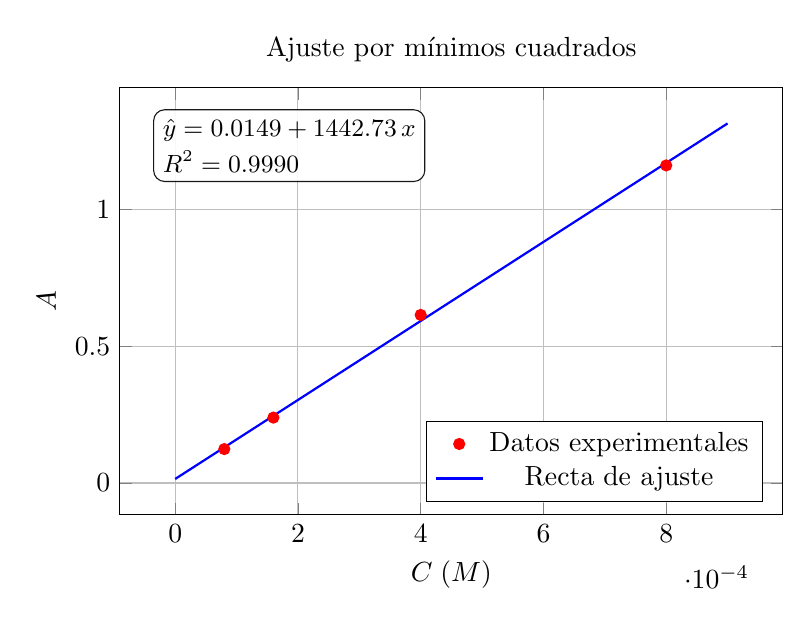
\begin{tikzpicture}
    \begin{axis}[
        grid=both,
        xlabel={$C\;(\text{M})$},
        ylabel={$A$},
        title={Ajuste por mínimos cuadrados},
        width=10cm,
        height=7cm,
        ticklabel style={/pgf/number format/fixed},
        legend style={at={(0.97,0.03)},anchor=south east},
    ]

    % --- Nube de puntos ---
    \addplot[
        only marks,
        mark=*,
        color=red,
        mark size=2pt
    ] coordinates {
        (0.00008, 0.124)
        (0.00016, 0.239)
        (0.00040, 0.614)
        (0.00080, 1.160)
    };
    \addlegendentry{Datos experimentales}

    % --- Recta de ajuste ---
    \addplot[
        domain=0:0.0009,
        samples=100,
        color=blue,
        thick
    ] {0.0148673 + 1442.73*x};
    \addlegendentry{Recta de ajuste}

    % --- Texto con ecuación y R^2 ---
    \node[anchor=north west, align=left, font=\small, fill=white, draw=black, rounded corners, opacity=0.9, text opacity=1]
        at (axis description cs:0.05,0.95)
        {$\hat{y} = 0.0149 + 1442.73\,x$\\[2pt]
         $R^2 = 0.9990$};

    \end{axis}
\end{tikzpicture}
    \caption{Ajuste por mínimos cuadrados}
\end{figure}
\bigskip
El coeficiente de correlación lineal \(r\) en notación de sumas es
\[
r=\frac{n S_{xy}-S_x S_y}{\sqrt{\big(n S_{xx}-S_x^2\big)\big(n S_{yy}-S_y^2\big)}}.
\]

Sustituyendo:
\[
\begin{aligned}
r &=\frac{4(0.00122176)- (0.00144)(2.137)}
{\sqrt{\big(4(8.32\times10^{-7})-(0.00144)^2\big)\big(4(1.795092999)- (2.137)^2\big)}}\\[6pt]
&\approx 0.9995008146.
\end{aligned}
\]

Finalmente,
\[
\boxed{R^2 = r^2 \approx (0.9995008)^2 \approx 0.9990019 \approx 0.9990.}
\]

\noindent Esto significa que aproximadamente el \(99.90\%\) de la variabilidad de \(A\) queda explicada por la concentración \(C\) mediante la recta de ajuste.


\bigskip
Como se pide la concentración para los datos de la tabla~\ref{tab:data-origin}
\begin{table}[H]\label{tab:data-origin}
    \centering
    \begin{tabular}{|c|c|c|}
        \hline
        n & Absorbancia $A$ & Concentración $C$ (M)\\
        \hline
        1 & $0.26$ & \\
        \hline
        2 & $0.46$ & \\
        \hline
        3 & $0.56$ & \\
        \hline
        4 & $0.85$ & \\
        \hline
        5 & $0.92$ & \\
        \hline
    \end{tabular}
    \caption{Datos que requieren la concentración de $\mathrm{K Mn O_4}$}
\end{table}

Utilizando la ecuación de la recta debemos despejar para $x$
\begin{equation*}
    x = \frac{A - 0.01487}{1442.72959}
\end{equation*}

Remplazando los datos para cada valor de $A$ obtenemos la siguiente tabla~\ref{tab:data-result}
\begin{table}[H]\label{tab:data-result}
    \centering
    \begin{tabular}{|c|c|c|}
        \hline
        n & Absorbancia $A$ & Concentración $C$ (M)\\ \hline
        1 & $0.26$ & $0.00017$ \\ \hline
        2 & $0.46$ & $0.00031$ \\ \hline
        3 & $0.56$ & $0.00038$ \\ \hline
        4 & $0.85$ & $0.00058$ \\ \hline
        5 & $0.92$ & $0.00063$ \\ \hline
    \end{tabular}
    \caption{Concentración de $\mathrm{K Mn O_4}$ para los datos de la tabla~\ref{tab:data}}
\end{table}